\section{Prosedur dan Algoritma Komputasi}

\subsection*{Alur Algoritma Komputasi Terintegrasi}
Prosedur pelaksanaan komputasi dirancang secara modular dan sekuensial yang terbagi ke dalam 7 tahapan kerja komputasi:
\begin{enumerate}
    \item \textbf{Tahap 1 (Akuisisi Data \& Pipeline CSV)}: Mengunduh data penampang lintang reaksi $^{12}\text{C}(n,\text{tot})$ dari repositori IAEA-NDS EXFOR via HTTP request. Jika koneksi jaringan mengalami gangguan, sistem secara otomatis mengaktifkan dataset kalibrasi terstandarisasi EXFOR 10224. Data ASCII mentah di-parsing menggunakan Regular Expression (\textit{Regex}) untuk mengekstrak tiga kolom presisi ganda ($E_i, \sigma_i, \Delta\sigma_i$), kemudian diekspor ke file CSV terformat.
    \item \textbf{Tahap 2 (Formulasi Analitik Gradien \& Hessian)}: Membangun modul fungsi penampang lintang Breit-Wigner, perhitungan residu terbobot $r_i$, fungsi objektif $\chi^2$, vektor gradien analitik $\mathbf{g}(\mathbf{p})$, dan matriks Hessian Gauss-Newton $\mathbf{H}(\mathbf{p})$ menggunakan operasi vektorisasi NumPy.
    \item \textbf{Tahap 3 (Ekstraksi Tebakan Awal Fisis)}: Menentukan vektor parameter awal:
    \begin{equation}
        \mathbf{p}_0 = \begin{bmatrix} E_r^{(0)} & \Gamma^{(0)} & \sigma_0^{(0)} & \sigma_{bg}^{(0)} \end{bmatrix}^T
        \label{eq:p0_init}
    \end{equation}
    berbasis data eksperimen: $E_r^{(0)}$ dari puncak spektrum ($\arg\max \sigma_i$), $\sigma_{bg}^{(0)}$ dari baseline tepi, $\sigma_0^{(0)}$ dari tinggi relatif puncak, dan $\Gamma^{(0)}$ dari estimasi FWHM.
    \item \textbf{Tahap 4 (Mesin Solver Newton-Raphson)}: Mengoperasikan loop iteratif pembaruan langkah $\mathbf{H}\Delta\mathbf{p} = -\mathbf{g}$ menggunakan fungsi pemecah dekomposisi LU (\texttt{np.linalg.solve}), mengevaluasi bilangan kondisi $\kappa(\mathbf{H})$ pada tiap langkah, dan menghentikan iterasi saat kriteria henti $\|\Delta\mathbf{p}\|_2 < 10^{-6}$ atau $|\Delta\chi^2| < 10^{-6}$ terpenuhi.
    \item \textbf{Tahap 5 (Evaluasi Statistik \& Kovariansi)}: Menghitung $\chi^2_{red} = \chi^2_{\min}/(N-4)$, matriks kovariansi $\mathbf{C} = 2\mathbf{H}^{-1}$, simpangan baku parameter $\delta p_j$, serta matriks korelasi silang $\boldsymbol{\rho}$.
    \item \textbf{Tahap 6 (Uji Ketahanan Numerik / \textit{Noise Stress-Test})}: Melakukan simulasi Monte Carlo dengan menginjeksikan derau Gaussian proporsional ($\sigma_{noisy} = \sigma + \mathcal{N}(0, \eta\sigma)$) pada level $\eta = 5\%, 15\%, 30\%$ untuk mengidentifikasi batas toleransi singularitas Hessian.
    \item \textbf{Tahap 7 (Visualisasi Saintifik \& Validasi Fisis)}: Membangkitkan kurva fitting kontinyu bersama titik eksperimen dan panel residu, memplot profil konvergensi kuadratik, serta memvalidasi kesesuaian nilai akhir $E_r$ terhadap literatur nuklir resmi.
\end{enumerate}
\newpage


\subsection*{Diagram Alir Pipeline Komputasi (\textit{Flowchart})}
Visualisasi diagram alir keseluruhan tahapan komputasi yang telah dirancang berbasis paket LaTeX TikZ disajikan pada Gambar~\ref{fig:flowchart}.

\begin{figure}[H]
    \centering
    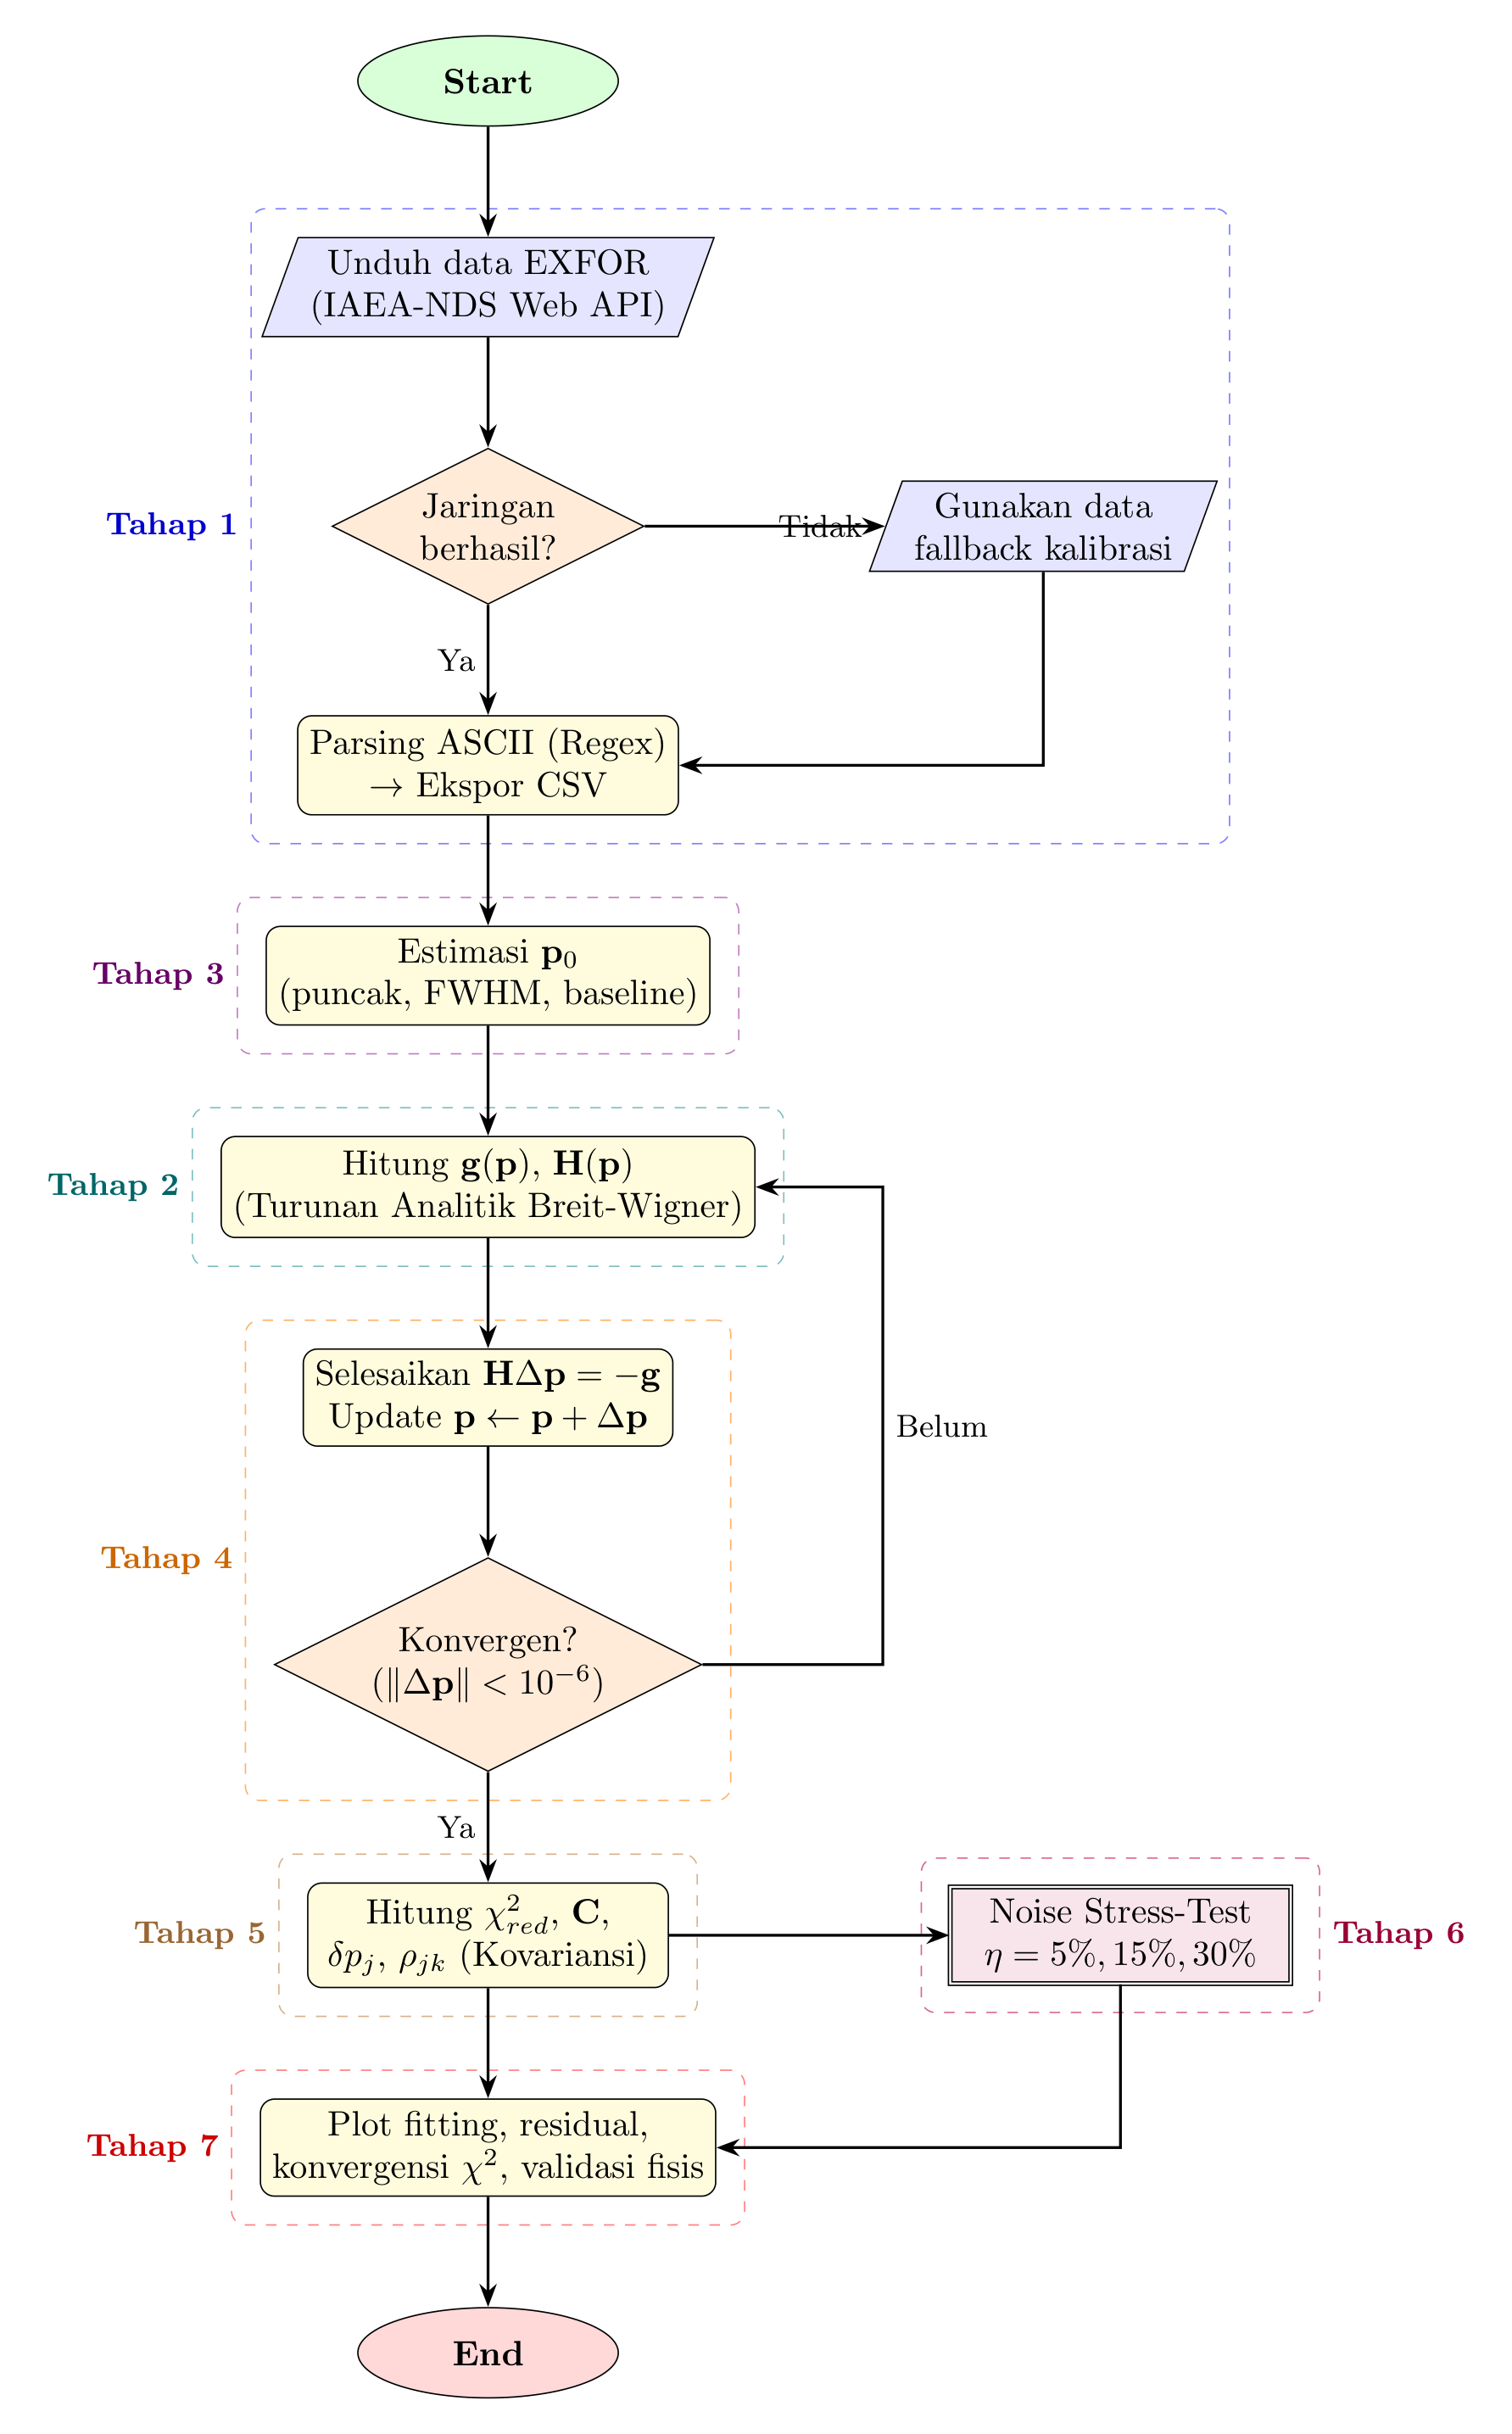
\includegraphics[width=0.62\textwidth]{flowchart_pipeline.png}
    \caption{Diagram alir (\textit{flowchart}) algoritma fitting resonansi Breit-Wigner menggunakan metode Newton-Raphson multivariat.}
    \label{fig:flowchart}
\end{figure}

\newpage

\subsection*{Pseudocode Algoritma Utama (\textit{MainPipeline})}
Representasi algoritmik tingkat tinggi dari keseluruhan pipeline komputasi dirumuskan sebagai berikut:

\begin{lstlisting}[caption={Pseudocode alur kerja utama pipeline komputasi fitting Breit-Wigner.}]
ALGORITHM MainPipeline(target="C-12", reaction="N,TOT"):
    # Tahap 1: Akuisisi Data
    raw_text = FetchEXFORRaw(target, reaction)
    IF raw_text GAGAL DIUNDUH:
        raw_text = FallbackCalibratedDataset()
    (E, sigma, dsigma) = ParseEXFORAscii(raw_text)
    ExportToCSV(E, sigma, dsigma, "exfor_c12_resonance.csv")

    # Tahap 3: Ekstraksi Tebakan Awal
    p0 = EstimateInitialGuess(E, sigma)

    # Tahap 4: Loop Newton-Raphson
    p = p0;  converged = False;  k = 0
    WHILE k < max_iter AND NOT converged:
        # Tahap 2: Turunan Analitik
        g = ComputeGradient(p, E, sigma, dsigma)
        H = ComputeHessian(p, E, sigma, dsigma)
        kappa = ConditionNumber(H)
        IF kappa > 1e12 OR det(H) <= 0:
            BREAK (Hessian ill-conditioned)
        delta_p = SolveLinearSystem(H, -g)
        p = p + delta_p
        IF norm(delta_p) < 1e-6 OR abs(delta_chi2) < 1e-6:
            converged = True
        k = k + 1

    # Tahap 5: Evaluasi Statistik
    chi2_red = ComputeChi2(p) / (len(E) - 4)
    Cov = 2 * InvertMatrix(H)
    delta_p = sqrt(diag(Cov) * chi2_red)
    rho = NormalizeCorrelation(Cov)

    # Tahap 6 & 7: Stress-Test & Visualisasi
    stress_results = RunNoiseStressTest(E, sigma, dsigma)
    PlotResonanceFitting(E, sigma, dsigma, p, delta_p)
    PlotConvergenceMetrics(history)
    ValidatePhysics(p[0], delta_p[0])
    RETURN p, delta_p, chi2_red, Cov, rho
\end{lstlisting}
